% English Reference Grammar
% By Dylan B. Mikus
% Spring 2014: 11-731

\documentclass[twocolumn]{article}

\usepackage{hyperref}
\usepackage{url}
\usepackage[utf8]{inputenc}
\usepackage{fancyvrb}
\usepackage{graphicx}

% Packages for formatting page, paragraph, and line layout/spacing
\usepackage{setspace}
\usepackage[top=1.0in, bottom=1.0in, left=1.0in, right=1.0in]{geometry}

\usepackage{enumerate, enumitem}
\usepackage{amsthm, amsmath}
\usepackage{datetime}

% defining variables
\setlength{\columnsep}{0.25in}
\setlength{\parskip}{1mm}

\newcommand{\linespacing}{
  \onehalfspacing
  % \doublespacing
}

% All of our custom commands and environments
% English Reference Grammar
% By Dylan B. Mikus
% Spring 2014: 11-731

\usepackage[utf8]{inputenc}

\usepackage{amsthm, amsmath}
% defining variables
\DeclareMathOperator*{\argmin}{arg\,min}
\DeclareMathOperator*{\argmax}{arg\,max}

% These are the commands that we load in and use elsewhere

%%%%%%%%%%%%%%%%%%%%%%%%%%%%%%%%%%%%%%%%%%%%%%%%%%%%%%%%%%%%%%%
%% These functions are for the grow-diag-final-and algorithm %%
%%%%%%%%%%%%%%%%%%%%%%%%%%%%%%%%%%%%%%%%%%%%%%%%%%%%%%%%%%%%%%%

\newcommand{\wrapSmall}[1]{
  \small
  #1
  \normalsize
}

% This function says that a spot (i,j) is aligned if it has some neighbor
% aligned and if the spot is aligned in either of the alignment vectors.
% As such, it is recursively defined.
\newcommand{\isAlignedFromGrow}{
  \begin{align*}
    g(A^{(k)}, & a^{(k)}, b^{(k)}, i, j) = \\
    & A^{(k)}_{i,j}
    \text{ if } (a_i^{(k)} = j
    \text{ or } b_j^{(k)} = i), \\
    & 0 \text{ otherwise}
  \end{align*}
}

% This function just computes all neighboring points (including diagonals) on a
% square grid.
\newcommand{\neighborsFunc}{
  \begin{align*}
    \texttt{neighbors}(i, j) = &
     \{
           \langle i-1, j   \rangle,
           \ \langle i  , j-1 \rangle,
           \ \langle i+1, j   \rangle,
           \ \langle i  , j+1 \rangle, \\
         & \langle i-1, j-1 \rangle,
           \ \langle i-1, j+1 \rangle,
           \ \langle i+1, j-1 \rangle, \\
         & \ \langle i+1, j+1 \rangle
     \}
  \end{align*}
}

% This function evaluates to true (1) if the given matrix point is in the
% intersection of the two alignment vectors.
% If the point is not in the intersection, then it evaluates to true (1)
% if the matrix point has some neighbor that is aligned, and that point is also
% in the union of the two alignment vectors (i.e., `g` evaluates to true), then
% we return true, otherwise we return false (0).
\newcommand{\isAlignedFromInterOrGrow}{
  \begin{align*}
    f(A^{(k)}, & a^{(k)}, b^{(k)}, i, j) = \\
      1 \text{ if }
         & (a_i^{(k)} = j \text{ and } b_j^{(k)} = i), \\
      \text{else } & \texttt{min}(1,
        \ |\{ \langle i', j' \rangle\ :\ i',j'
            \in \texttt{neighbors}(i,j) \\
         &~~~~ \text{ and } g(A^{(k)}, a^{(k)}, b^{(k)}, i', j') = 1 \}|)
  \end{align*}
}


\newcommand{\growDiagMatrix}{
  \begin{align*}
    A^{(k)}_{i,j} = \text{ case } & f(A^{(k)}, a^{(k)}, b^{(k)}, i, j) \text{ of } \\
        & 1 \Longrightarrow 1 \\
        & 0 \Longrightarrow (1 \text{ if } a^{(k)}_i = j
                               \text{ or } b^{(k)}_j = i)
  \end{align*}
}


%%%%%%%%%%%%%%%%%%%%%%%%%%%%%%%%%%%%%%%%%%%%%%%%%%%%%%%%%%%%%%
%% These functions are for the phrase-based-align algorithm %%
%%%%%%%%%%%%%%%%%%%%%%%%%%%%%%%%%%%%%%%%%%%%%%%%%%%%%%%%%%%%%%

% Creates a sequence with the middle elements collapsed.
\newcommand{\seqSpan}[2]{
  \langle #1 \cdots #2 \rangle
}

% where $c(e)$ counts the number of occurrences of phrase $e$ in training,
% and $c(e,f)$ counts the number of phrase pairs $(e,f)$ in training.
\newcommand{\phrasePairNorm}{
    C(\overline{e},\overline{f})
      = \frac{c(\overline{e},\overline{f})}
              {c(\overline{e})}
}

% This function gets all possible phrases in e, all possible phrases in f, and
% the normalized frequency counts for those phrase pairs.
\newcommand{\allPhrasePairs}{
  \begin{align*}
    P =
      \large\{
        (e_i, & e_j, f_m, f_n,
          C(\seqSpan{e_i}{e_j},\ \seqSpan{f_m}{f_n})) \\
        \ &:\ 0 \leq i \leq j \leq \texttt{len}(e),
           \ 0 \leq m \leq n \leq \texttt{len}(f)
      \large\}
  \end{align*}
}

% This evaluates to the most probable set of phrase pairs that cover the
% entirety of the source sentence f and the target sentence e.
\newcommand{\optPhraseCoverage}{
\begin{align*}
    h(e,f&) = \\
    & Q \subset P \text{ such that } \forall x_1, x_2 \in Q \text{ where } \\
        & \hspace{0.35in} x_1 = (e_i, e_j, f_m, f_n, C(\seqSpan{e_i}{e_j},
                                    \seqSpan{f_m}{f_n})) \\
        & \hspace{0.35in} x_2 = (e'_i, e'_j, f'_m, f'_n, C(\seqSpan{e'_i}{e'_j},
                                        \seqSpan{f'_m}{f'_n})), \\
        & \hspace{0.2in} (\seqSpan{e_i}{e_j}
                                        \cap \seqSpan{e'_i}{e'_j} = \emptyset \\
        & \hspace{0.2in} \text{ and } \seqSpan{f_m}{f_n}
                                        \cap \seqSpan{f'_m}{f'_n} = \emptyset) \\
        & \hspace{0.05in} \text{ and such that }
                             \forall y \in \seqSpan{e_0}{\texttt{len}(e)}, \\
        & \hspace{0.925in}   \forall z \in \seqSpan{f_0}{\texttt{len}(f)} \\
        & \hspace{0.35in} \exists x_3 \in Q, x_3 = (e''_i, e''_j, f''_m, f''_n, \\
        &~~~~~~~~~~~~~~~~~~~~~~~~~~~~~ C(\seqSpan{e''_i}{e''_j},
                                   \seqSpan{f''_m}{f''_n})) \\
        & \hspace{0.45in} \text{ such that } e''_i \leq y \leq e''_j, f''_m \leq z \leq f''_n \\
        \vspace{0.5in}
        & \argmax_{Q \subset P} ( Q \text{ for } \sum_{q \in Q} q.\texttt{prob} )
  \end{align*}
}


\newcommand{\growPhraseMatrix}{
  \begin{align*}
    B_{i,j}^{(k)} = \text{ case } & h(e,f) \text{ of } \\
        & \emptyset \Longrightarrow A_{i,j}^{(k)} \\
        & Q \Longrightarrow 1 \text{ if } \exists x \text{ where }
            x = (\langle e_a, e_b \rangle,
                 \langle f_c, f_d \rangle, p) \\
            & \hspace{.5in} \text{ such that } a \leq i \leq b \text{ and } c \leq j \leq d \\
            & \hspace{.4in} 0 \text{ otherwise}
  \end{align*}
}


\newcommand{\intersectMatrix}{
  \begin{align*}
    C_{i,j}^{(k)} = & 1 \text{ if } (A_{i,j}^{(k)} = 1) and (B_{i,j}^{(k)} = 1) \\
                 & 0 \text{ otherwise}
  \end{align*}
}


% Local Variables:
% mode: latex
% End:

\newcommand{\originalAlign}{\texttt{grow-diag-final-and}}
\newcommand{\phraseAlign}{\texttt{from-phrase-table}}
\newcommand{\phraseIntersectAlign}{\texttt{grow-intersect-phrase}}
\newcommand{\wrapSingleSpacing}[1]{
  \singlespacing
  #1
  \linespacing{}
}


\title{Alignment Matrix Generation Based on Phrases \\
  11-731: Machine Translation, Spring 2014}
\date{\today}
\author{Dylan Bergeron Mikus}

\begin{document}
% Instructions:
% - Explain your implementation and evaluation.
% - Discuss prior and related work.
% - Analyze your results.
% - Answer the question: what did you learn?
\maketitle{}

\begin{center}
\Large{\textbf{Abstract}}
\end{center}
\begin{quotation}
  \small{
    This report proposes a new word alignment model for phrase-based
    translation. Traditionally, when generating our phrase table during
    training, we align words based on a lexical model with some applied
    heuristics (using GIZA++, for example). The phrase-based MT system then uses
    these alignment matrices to generate a phrase table.
    We propose an alignment method called \phraseIntersectAlign{} that runs a
    standard word alignment algorithm, but then attempts to re-align words based
    on the phrase-table output from the first alignment, and then intersect
    these two alignment matrices. We find the optimal set of phrase pairs that
    cover an entire (source, target) sentence pair, and then align every word
    within a source phrase to every word in its corresponding target phrase.
    We use Moses for conducting experiments, and all other phrase-based MT steps
    remain standard. Our new system does not show any improvement or decline in
    BLEU score, but given the room for improvement and similar promising
    research, it is possible that this approach can net positive results with
    future work.
  }
\end{quotation}


\section{Introduction}
In phrase-based translation, we extract phrases based on alignment matrices
generated for each sentence. There are a number of methods for aligning the
words between parallel sentences. For the most part, these all depend on
alignment from hidden Markov models, or IBM models with a few additional
heuristics applied. Research (\cite{wuwang2007}, \cite{dgzk2006}) has shown that
heuristic models applied on top of traditional word-alignments for alignment
matrix generation results in improved phrase translation and higher evaluation
scores.

In state of the art translation systems, phrase-based alignment performs better
than word-based alignment. So, we want to determine if this improvement relation
holds for the alignment matrix generation step. Specifically, we evaluate the
translation quality of a system that uses phrases for the generation of
alignment matrices. After generating a phrase table based on standard alignment
matrix generation and phrase extraction, we go back and reapply the phrase table
to generating new alignment matrices. We call this method \phraseAlign{}.
Then we intersect the \phraseAlign{} matrices with the original alignment
matrices. These are called the \phraseIntersectAlign{} matrices.
Our hope is that \phraseIntersectAlign{} will remove outlying alignment points
that are errors from the word and heuristic based alignment matrix generation.

For our experiments, we use parallel corpus data from the
\href{http://www.statmt.org/wmt13/training-parallel-nc-v8.tgz}
     {\underline{www.statmt.org/wmt13}}
Workshop on Statistical Machine Translation.
Our experiments show that no perceivable improvement in BLEU score, but also no
degradation of BLEU score. Given the additional runtime imposed by re-aligning
based on phrases, we consider this a negative result, but believe that there is
room for improvement in both the runtime speed of training under the
\phraseIntersectAlign{} method, and potentially for the overall translation
accuracy.


\section{Background}
\subsection{Phrase-Based Translation}
Phrase-based statistical machine translation is largely the front-running
machine translation method. A standard phrase-based translation system can be
divided into a number of distinct steps:
\wrapSingleSpacing{
\begin{enumerate}
    \item language model training
    \item alignment matrix generation
    \item phrase extraction
    \item translation model training
    \item phrase-based sentence decoding and translation
\end{enumerate}
}
The language model is typically a set of n-gram frequencies (possibly unigram,
bigram, and trigram), summed up across the whole training corpus and then
normalized. Then an IBM model or hidden Markov model for word alignment uses the
language model to align words from source sentences to target sentences and vice
versa. Traditionally, one then applies heuristics on top of these two alignments
to generate a final alignment matrix.
Most alignment methods use an unsupervised approach, employing software such as
Giza++.

There has also been work with semi-supervised models, such as work by
Pal et al. \cite{pnb2013}, which uses named-entity taggers to align named
entities to one another, and then creates chunks based on grammatical
rules. They attempt to align the chunks to one another using fuzzy matching on a
baseline SMT model. After aligning chunks, words within chunks matching chunks
are aligned to each other. This is quite similar to our method, but employs
grammatical rules instead of strictly unsupervised phrase-based translation, and
it uses fuzzy matching instead of an exact and non-overlapping set of
(source, target) phrase pairs. The experiment saw significant improvement in
the BLEU score from the baseline using Giza++ and
\originalAlign{}. \cite{pnb2013}.

% mathematical model for word alignment translation and stuff
For a given target sentence $e$ of length $m$, source sentence $f$ of length
$n$, and alignment $a$ from $f$ to $e$ for every $e_i \in e$, the probability of
a given translation is:
\[
  p(e | f, m) = \sum_{a \in [0, n]^m} p(a | f,m)
    \times \prod_{i=1}^m p(e_i | f_{a_i})
\]
Then for the max alignment vector $a$ combined with the language model results
according to the alignment, we can use $a$ to make our alignment
matrix. Typically, we will generate alignments from $f$ to $e$ and from $e$ to
$f$ and then apply a heuristic somehow combining these alignments.
For more information on phrase-based MT, Koehn et al. \cite{kom2003}'s paper
gives a more substantial description of all the steps involved.

For our project, we use the Moses phrase-based MT system to run the components
of the system. To generate alignment vectors, Moses uses GIZA++. The default
heuristic applied to these vectors is called \originalAlign{}.
Firstly, we use a superscript notation $(k)$ to represent the $k^{\text{th}}$
sentence in the source and target corpus.
For the $k^{\text{th}}$ sentence pair, we define two alignment vectors, one for
each direction:
\[ a^{(k)} = \argmax_a p(f^{(k)}, a\ |\ e^{(k)}, m_k) \]
\[ b^{(k)} = \argmax_b p(e^{(k)}, b\ |\ f^{(k)}, n_k) \]
We have an alignment matrix $A^{(k)}$, where cell $(i,j)$ is $1$ if word $e_i$
and $f_j$ are aligned, and $0$ otherwise.
We define the qualifications for alignment in the following manner:

$g$ says that a matrix cell $(i,j)$ is aligned if it has an aligned
neighbor and if the cell is aligned in either of the alignment vectors
$a^{(k)}$ or $b^{(k)}$.
As such, it is recursively defined based on following functions.
\wrapSmall{\isAlignedFromGrow{}}


This function just computes all neighboring points (including diagonals) in a
matrix.
\wrapSmall{\neighborsFunc{}}

$f$ evaluates to 1 if the given matrix point is in the
intersection of the two alignment vectors.
If the point is not in the intersection, then it evaluates to 1
if the matrix point has some neighbor that is aligned, and that point is also
in the union of the two alignment vectors (i.e., `g` evaluates to 1), then
we return 1, otherwise we return 0.
\wrapSmall{\isAlignedFromInterOrGrow{}}

Ultimately, we define each cell in the matrix such that
the cell evaluates to 1 if the it is in the
intersection of both alignment vectors, if it is not in the intersection but is
in the union of the two alignment vectors and neighbors a previously aligned
cell, or finally if the spot was not yet aligned but is in the union of the two
alignment vectors. This has the effect of preferring alignments grown from the
intersection before finally falling back on the union of alignments.
\wrapSmall{\growDiagMatrix{}}


So, the algorithm starts with the intersection of the alignment vectors, and
then grows out to neighbors that are aligned in the union of the two vectors,
$a^{(k)}$ and $b^{(k)}$.

For pseudo-code for \originalAlign{}, see figure \ref{fig:growDiagPseudo}.

\begin{figure*}[t]
\begin{Verbatim}[frame=single]
GROW-DIAG-FINAL(e2f,f2e):
  neighboring = ((-1,0),(0,-1),(1,0),(0,1),
                 (-1,-1),(-1,1),(1,-1),(1,1))
  alignment = intersect(e2f,f2e);
  GROW-DIAG(); FINAL(e2f); FINAL(f2e);

 GROW-DIAG():
  iterate until no new points added
    for english word e = 0 ... en
      for foreign word f = 0 ... fn
        if ( e aligned with f )
          for each neighboring point ( e-new, f-new ):
            if ( ( e-new not aligned or f-new not aligned ) and
                 ( e-new, f-new ) in union( e2f, f2e ) )
              add alignment point ( e-new, f-new )
 FINAL(a):
  for english word e-new = 0 ... en
    for foreign word f-new = 0 ... fn
      if ( ( e-new not aligned or f-new not aligned ) and
           ( e-new, f-new ) in alignment a )
        add alignment point ( e-new, f-new )
\end{Verbatim}
\caption{Pseudo-code for \originalAlign{}}
\label{fig:growDiagPseudo}
\end{figure*}

%% \subsection{Prior Work}

%% \subsection{Related Work}

\section{Evaluation Methods}
\subsection{Translation Model}
We use the standard phrase-based translation model and a lexical language
model (see above for the language model).
Using Bayes rule, we can rewrite the probability for translating from a
foreign sentence $f$ to a target sentence $e$ as:
\[
  \argmax_e p(e|f) = \argmax_e p(f|e) p_{\text{LM}}(e)
\]
We have the translation model probability $p(f|e)$, and the language model
probability for the target sentence $p_{\text{LM}}(e)$.
The language model is based on n-gram frequency, usually tri-gram.
The translation model decomposes further. During the decoding
process, we separate the foreign sentence $f$ into a series of foreign phrases,
$\overline{f}_i$, and then each $\overline{f}_i$ translates into an target
phrase $\overline{e}_i$. The probability of this translation for a given phrase
pair $(\overline{e}_i, \overline{f}_i)$ is, by Bayes rule, this translation
model (ignoring alignment at this point) has the probability distribution
$\phi(\overline{f}_i, \overline{e}_i)$.


Then, given a sequence $a$, where $a_i$ is the start position of the foreign
phrase that translates into the $i$th target phrase,
and another sequence $b$ where $b_i$ is the end position of the foreign phrase
that translates into the $i$th target phrase,
we define a function $d(a_i - b_{i-1})$ that negatively weights against
alignments that reorder. This is heuristic based, but in general, most sentences
share similar order with their translations. $\omega$ is a real number
parameter used counter-balance against the preference for shorter sentences.
If $I$ is the set of foreign phrases that cover the foreign sentence $f$, then
the probability for the translation model can be summarized as:
\begin{align*}
  \argmax_e p(e|f) & = \\
      & \argmax_e p(f|e) p_{\text{LM}}(e) \omega^{\text{len}(e)} = \\
      & \argmax_e p_{\text{LM}}(e) \omega^{\text{len}(e)}
                  \prod_{i=1}^I \phi(\overline{f}_i | \overline{e}_i)
                              d(a_i - b_{i})
\end{align*}
Please refer to \cite{kom2003} for a more detailed description of the model.


\subsection{Evaluation Components}
We record a number of different values to use during our evaluation.
Let $S_0$ be the phrase table generated by \originalAlign{}.
Let $S_1$ be the phrase table generated by \phraseIntersectAlign{}
These include:
\wrapSingleSpacing{
\begin{enumerate}
  \item the number of alignment points removed from
    the \originalAlign{} alignment matrix
    by intersection with
    the \phraseAlign{} alignment matrix.
  \item $s_0 = |S_0|$
  \item $s_1 = |S_1|$
  \item $s_2 = |S_0 \cup S_1|$
  \item $s_3 = |S_0 \cap S_1|$
\end{enumerate}
}

To evaluate the results, we use a number of different metrics, we ultimately
concern ourselves with the difference between the BLEU score from using Moses
phrase-based translation with alignment matrices generated from \originalAlign{}
and the BLEU score from using Moses phrase-based translation with alignment
matrices generated from \phraseIntersectAlign{}.

To dig a little deeper and gain empirical data that can help us understand our
results, we will also look at the differences in the phrase tables and alignment
matrices. We will use the phrase-table size information in the above list, as
well as computing the fraction of alignment points removed from the
\originalAlign{} by intersecting with \phraseIntersectAlign{}.

It is our hypothesis that \phraseIntersectAlign{} will remove outlying
points that never happen to fall into the most common or probable phrases. This
may have a positive effect on the overall BLEU score, or it might have a
negligible effect on the BLEU score, but it should at least still decrease the
size of our phrase table without much harm to future decoding. This has the
potential to speed up the decoding process for phrase-based translation.

For our test set, we use unique corpora within
The Workshop on Statistical Machine Translation 2012 dataset,
available at
\href{http://www.statmt.org/wmt12/dev.tgz}
     {\underline{www.statmt.org/wmt12}}.


\section{Implementation}
There are two parts to the process of generating alignment matrices based on
phrases. First off, we run the full process of phrase-based translation using
the \originalAlign{} method. Using Giza++ for lexical alignment and the Moses MT
system to run the whole translation process (incorporating alignment from
Giza++), we evaluate phrase-based decoding and evaluation against a set of
testing data using the BLEU scoring metric. This gives us our baseline data for
the system based on the defaults for a Moses experiment.

After we have a phrase table generated for our training data, we can create an
alignment matrix using the following idea: if phrase $f_i$ is aligned to phrase
$e_j$, then we align every word in $f_i$ to every word in $e_j$. We define the
final alignment matrix as the intersection of this phrase-based alignment matrix
and the traditional lexical alignment matrix.


%%%%%%%%%%%%%%%%%%%%%%%%%%%%%%
%% Figures from experiments %%
%%%%%%%%%%%%%%%%%%%%%%%%%%%%%%

\begin{figure*}[tbp]
  \setlength{\tabcolsep}{12pt}
  \begin{tabular}{c c c}
      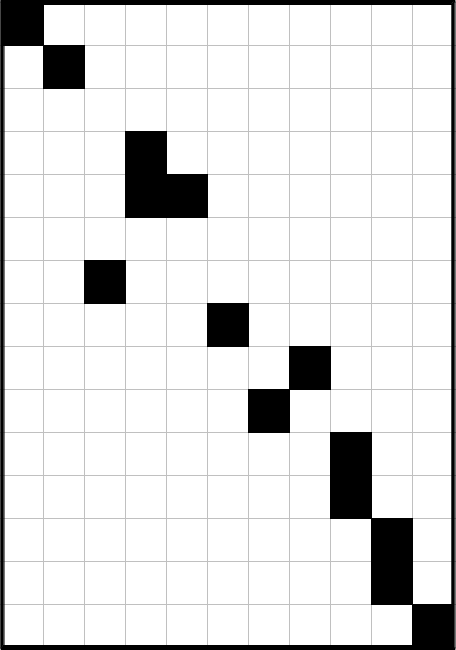
\includegraphics[scale=0.4]{imgs/grow-diag-final-and-align.png}
    & 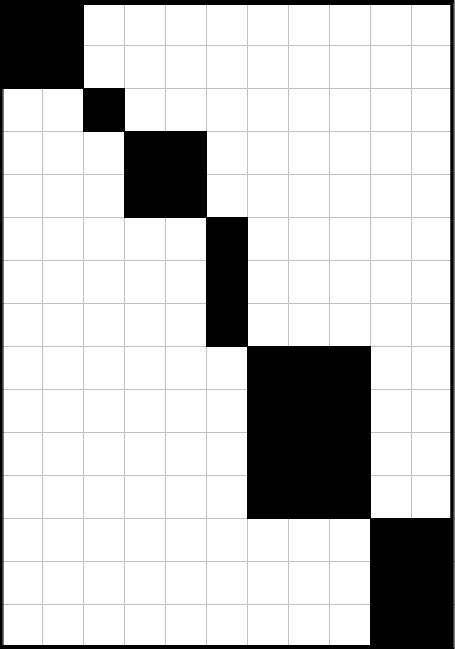
\includegraphics[scale=0.4]{imgs/phrase-align.png}
    & 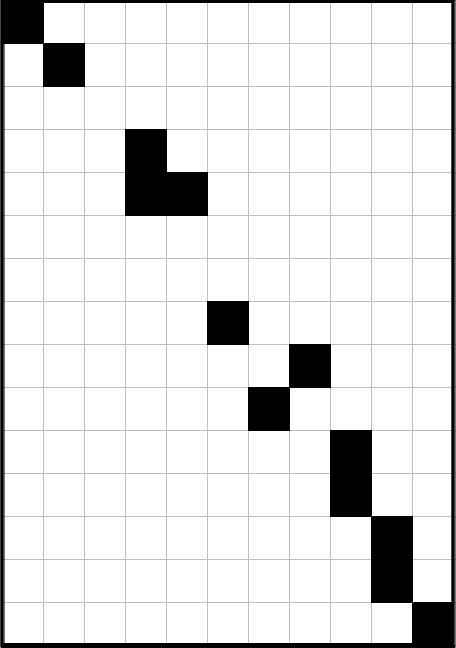
\includegraphics[scale=0.4]{imgs/phrase-intersect-align.png} \\
    %
      \originalAlign{}
    & \phraseAlign{}
    & \phraseIntersectAlign{}
  \end{tabular}
  \begin{center}
    Rows are English words.

    Columns are French words.

    English sentence is:
    ``One answer , of course , is a complete collapse of the US dollar .''

    French sentence is:
    ``Une r\'{e}ponse est bien s\^{u}r un effondrement complet du dollar .''
  \end{center}
  \caption{Example word alignment matrices for different alignment methods.}
  \label{fig:alignMatrices}
\end{figure*}

\begin{table*}[tbp]
  \begin{center}
    \begin{tabular}{| l | l | l | l |}
      \hline
      Method  &  Test File Name  &  BLEU Score  &  Phrase Table Size \\
      \hline
      \originalAlign{} (baseline)  &  newstest2010  &  18.11  &  2,105,246 \\
      \hline
      \phraseIntersectAlign{}  &  newstest2010  &  18.11  &  2,174,330 \\
      \hline
    \end{tabular}
  \end{center}
  \caption{Experiment numerical results}
  \label{table:expResults}
\end{table*}

%%%%%%%%%%%%%%%%%%%%%%%%%%%%%%%%%%%%%%%%
%% Done with figures from experiments %%
%%%%%%%%%%%%%%%%%%%%%%%%%%%%%%%%%%%%%%%%


\subsection{Generating New Alignment Matrices}
Simply put, \phraseAlign{} finds the most probable set of
(English prefix, French coverage vector) pairs that covers all of the English
sentence $e$ and the French sentence $f$. The algorithm then aligns all words to
one another within corresponding (English, French) pairs. However, if we are
unable to cover the entirety of $e$ and $f$, we fall back to the original
alignment from \originalAlign{}. Furthermore, for performance reasons, if a
French sentence is over a certain length, we fall back to the original alignment
matrix. This is due to the fact that finding an optimal coverage phrase set for
English and French is computationally expensive.

Specifically, the \phraseAlign{} algorithm works as follows:
\wrapSmall{\[ \phrasePairNorm{} \]}
where $c(\overline{e})$ counts the number of occurrences of phrase
$\overline{e}$ in training,
and $c(\overline{e},\overline{f})$ counts the number of phrase pairs
$(\overline{e},\overline{f})$ in training. \\

We then compute the set, $P$, of all possible phrase pairs for $e$ and $f$,
along with the normalized frequencies for those phrase pairs.
\wrapSmall{\allPhrasePairs{}}

In set $P$ we must find the most probable set of phrase pairs that cover the
entirety of the source sentence $f$ and the target sentence $e$. We define $Q$
as a subset of $P$, where the phrase pairs in $Q$ cover all of $f$ and $e$.
We must take the most probable coverage pair set possible. Note that our source
code does not exhaustively generate all possible subsets, but instead generates
them subsets preferring more probable phrases first and returning early if we
find a phrase set that covers $f$ and $e$. We define this function $h$ as:
\wrapSmall{\optPhraseCoverage{}}

Finally, at the root of the algorithm, we attempt to find a set $Q$. If such a
set exists, the we align every word in $\overline{e}_i$ to every word in
$\overline{f}_i$. If no set $Q$ exists, we fall back to the alignment matrix
from \originalAlign{}. Define the new alignment matrix for \phraseAlign{} as:
\wrapSmall{\growPhraseMatrix{}}

The we simply define the matrix $C^{(k)}$ for \phraseIntersectAlign{}
as the intersection of $A^{(k)}$ and $B^{(k)}$:
\wrapSmall{\intersectMatrix{}}

If you wish to see the code for this algorithm, please refer to
the function \verb!phrase_alignment(f, e, tm, k)!
in the file \verb!align_from_phrases.py!.
You can locate this content at
\href{https://github.com/dbmikus/11-731.phrase-matrix-aligner}
     {\wrapSmall{\underline{https://github.com/dbmikus/11-731.phrase-matrix-aligner}}}.

\section{Experiments and Results}
\subsection{Experimental Setup and Process}
We used a training corpus from
\href{http://www.statmt.org/wmt13/training-parallel-nc-v8.tgz}
     {\underline{www.statmt.org/wmt13}}.
This news commentary corpus consists of over 100,000 (English, French) parallel
sentences.
We initially limited the corpus to 100,000 parallel sentences, but the
combined required computing power to store the translation model and find
optimal (English, French) phrase-based coverage vectors took far too long.
Then we truncated the parallel sentence corpus to 25,000 sentences.
As part of the Moses SMT pipeline, we tokenized and cleaned the input, limiting
maximum sentence length to 80 words. This reduced the size of the training
corpus by a small amount.
Training on a corpus of this size ran in reasonable time. Note that
Pal et al. \cite{pnb2013},
who ran a related experiment, also uses a relatively small training corpus,
containing 22,492 parallel sentences. This may be due to their use of (Bengali,
English) pairing, or it may also stem from performance reasons, but it is worth
noting.

For evaluation we used a test corpus of English and French parallel sentences
from The Workshop on Statistical Machine Translation 2012. We used 3,003
sentence pairs.

We used a 3-gram language model, and limited phrase length to a maximum of 4
words per phrase. In the translation model,
for each French phrase $\overline{f}$, we
limited the size of the possible corresponding English phrases to the maximum
integer size on our machine, which was a very large number. Needless to say,
this did not appear to be a restricting value.

Due to performance issues and the computational complexity of finding the
optimal set of French and English phrases to cover a parallel sentence pair
$(f, e)$, we had to impose some restrictions on the phrase-alignment generator.
We only searched for a phrase-based alignment if a sentence was under 20 tokens
long.
Also, for a given sentence, when we generated the list
\texttt{alignments}, with \texttt{alignments[i]} being
an inner list of all the phrases in $f$ that could have generated phrases
starting at position \texttt{i} in $e$, we limited the number French phrases per
English starting point to the 500 most probable.
With these parameters, the training and evaluation ran in a reasonable time.


\subsection{Results}
Interestingly, the BLEU scores for \originalAlign{} and \phraseIntersectAlign{}
were both 18.11. And contrary to our hypothesis, the phrase table generated from
the \phraseIntersectAlign{} matrices was just under 70,000 entries larger than
the phrase table from \originalAlign{}. This could be because outlying points in
the original alignment matrices interfered with certain phrase possibilities,
rendering those phrases inconsistent. When we removed these points, perhaps we
were able to extract a greater number of consistent phrases.
Refer to \ref{table:expResults} for the experimental results breakdown.

%% NUMBER of correctly aligned = 4572
%% NUMBER unable to align = 1940
%% NUMBER too long, so fast aligned = 18211
%% NUMBER of total sentences = 24723
%% NUMBER matrix alignment points removed = 4300
In the training set, we had 24,723 sentence pairs.
\begin{itemize}
  \item 73.66\% of the sentences were too long for us to re-align using phrases.
  \item Of the remaining 26.34\% of the sentence pairs, we were able to
    successfully re-align sentence pairs 70.21\% of the time
  \item 18.49\% of the total sentence pairs could be successfully re-aligned
    based on phrases
\end{itemize}
This data indicates that about 3/4 of the sentence pairs in the training corpus
did not pass through the attempt at phrase-based alignment. As stated above, we
did try to increase the limit on maximum sentence length, but we ran into
performance issues.

The intersection between \originalAlign{} and \phraseAlign{} removed, in total,
4,300 points that were aligned by \originalAlign{} matrices. Overall, it
appeared that \phraseAlign{} tended to align strongly along the diagonal, so the
intersection could drop alignment points that were further from the
diagonal. See \ref{fig:alignMatrices} for an example of the three alignment
matrices.

Looking at the phrase tables,
let $PT_1$ be the table generated from \originalAlign{}
and $PT_2$ be the table generated from \phraseIntersectAlign{}.
\begin{itemize}
  \item $|PT_1| = 2,105,246$
  \item $|PT_2| = 2,174,330$
  \item $|PT_1 \cap PT_2| = 2,104,072$
  \item $|PT_1 \cup PT_2| = 2,175,504$
  \item $|PT_1 - PT_2| = 1,174$
  \item $|PT_2 - PT_1| = 70,258$
\end{itemize}

%% Yes - I suggested measuring the impact on the phrase tables by looking at the
%% fraction of phrases that are in the intersection, and also the fraction of
%% phrases that are in one system but not in the other.  You can do this
%% globally, on the entire phrase table, or you can do this at the level of the
%% phrases available for decoding individual sentences in the test set (or
%% accumulate the stats for the entire test set).  The latter is likely more
%% difficult to implement.

%% Your idea of running statistics on the fraction of alignment cells that are
%% removed when intersecting the matrices is also a good idea.

%% Given that time is very limited at this point, I think the above would be
%% sufficient.

%% Looking forward to seeing your final results and reading your report!

\section{Conclusion}
From the results of our experiment, we cannot conclude that the
\phraseIntersectAlign{} method for generating word alignment improves any
translation results. In fact, given the performance hit that a system undergoes
by adding this additional component to the training system, one could conclude
that the results of the \phraseIntersectAlign{} method are negative.
However, there are a few obvious improvements to implement that could lead to
more comprehensive data and testing. In future experiments, we must improve the
speed the algorithm that attempts to create a fully covered mapping between
given $(f, e)$ pairs. The current algorithm performs a rather exhaustive search
on the sentence pair to find the optimal phrase-based alignment. It uses dynamic
programming to backtrack and find the most probable set of phrase pairs that
lead to a given English prefix and French coverage vector.
We could instead employ some heuristics and make the alignment a little more
fuzzy, perhaps choosing the most probable phrase starting at the first index,
then the most probable phrase starting at the point after that, and so on,
filling in the gaps with lexical alignment values from \originalAlign{}.

If we could speed up the \phraseAlign{} method, then we would be able to run
\phraseAlign{} on larger sentences and larger corpora. Given the limited
percentage of the corpus that \phraseAlign{} ran on, it is possible that the
method either improved or decreased the BLEU score, but any changes were small
enough to be drowned out by the number of sentences for which we fell back to
the standard \originalAlign{} alignment method. Given the success of
similar research by Pal et al. \cite{pnb2013}, with a combined unsupervised and
semi-supervised alignment system, it should be worth it to investigate improving
the algorithms and methods outlined in this report.


\begin{thebibliography}{99}
  \bibitem{wuwang2007}
    Wu, Hua and Wang, Haifeng
    (2007).
    Comparative Study of Word Alignment Heuristics and Phrase-Based SMT.
    In \emph{Toshiba (China) Research and
      Development Center}.

  \bibitem{dgzk2006}
    DeNero, John and Gillick, Dan and Zhang, James and Klein, Dan
    (2006).
    Why Generative Phrase Models Underperform Surface Heuristics.
    In \emph{Proceedings of the Workshop on Statistical Machine Translation}.

  \bibitem{kom2003}
    Koehn, Philipp and Och, Franz Josef and Marcu, Daniel
    (2003).
    Statistical Phrase-Based Translation.
    In \emph{Proceedings of HLT-NAACL}.

  \bibitem{mt11731}
    Dyer, Chris and Lavie, Alon
    (2014).
    11-731: Machine Translation.
    \href{http://demo.clab.cs.cmu.edu/sp2014-11731/}
     {\underline{http://demo.clab.cs.cmu.edu/sp2014-11731/}}.
    In Carnegie Mellon University curriculum.

  \bibitem{collins2013}
    Collins, Michael
    (2013).
    Phrase-Based Translation Models.
    From Columbia University CS Department.

  \bibitem{pnb2013}
    Pal, Santanu and Naskar, Sudip Kumar and Bandyopadhyay, Sivaji
    (2013).
    A Hybrid Word Alignment Model for Phrase-Based Statistical Machine
    Translation.
    In \emph{Proceedings of the Second Workshop on Hybrid Approaches to
      Translation}.
\end{thebibliography}
\end{document}

% Local Variables:
% mode: latex
% fill-column: 80
% eval: (auto-fill-mode 1)
% End:
